\chapter{Custom Parts}

\textbf{Author: Fabian Kleinrad} 

This chapter is going to take a look at the practical side of the autumn project. When working with hardware there is the inevitable need for parts fit for the underlying application. In the case of autumn, with the Matrice 100 being in the centre of the project the need arises to design and manufacture parts in order to make the hardware portion in autumn come together without any complication and potential weak points in the final product.

\section{Reasons}

The goal of the autumn project being as innovative and unique in terms of methods used in the realization of the project, parts needed are either not readily available or not compliant with the budget. Another difficulty is parts are too specific for there to be any commercially available. Therefore to guaranty the reusability and reliability of the final product, methods to design and produce parts specifically tailored to the needs in the autumn project have to be utilized.

\subsection{Camera Mount}

Autumn conquers the problem of mapping an environment with the use of a drone. Therefore it is necessary to attach the camera used to capture the surroundings to the drone that allows it to move through that space. In the case of autumn, the camera being used is a ZED2i, which needs to be securely attached to a Matrice 100. Additionally to the cost factor and accompanying risk of damaging the hardware in use, the positioning and angle are important properties to consider. For that reason, a commercial solution is precluded.

\subsubsection{First approach}

When working under the principle of fast prototyping, the drawbacks of the first approach being incomplete is inherent. Following this principle lead to attaching the ZED2i to the Matrice 100 with the help of zip ties. The rationale for this decision was the reliability and strength of zip ties which allowed the camera to be secured tightly. This was important because of the need to test segments of the autumn project, worked on separately and isolated from one another. Taking simple and easy to realize steps enables the project to progress more smoothly and without the need for other sub-areas to be set on hold because of long tedious planning and manufacturing periods of parts like a custom camera mount for a drone.

\subsubsection{Problems without a Mount}

After a period of testing with a prototype, problems arise with the need for correction. In the case of, what most people consider a work-around rather than a solution to the problem of mounting a camera, they can be, in the case of this application, divided into two categories.
\newline The first aspect to consider when mounting a camera to a drone is its field of view. With UAVs hovering above ground a downward pointing angle is needed in order to be able to capture details close to the ground.  

\begin{figure}[h]
	\centering
	\includesvg[width=0.7\linewidth]{img/svg/FieldOfView}
	\caption{Depiction of the FOV for cameras mounted at different angles on a drone.\newline A: camera mounted vertically, B: camera mounted with a downward pointing angle.}
	\label{fig:custom_parts_FOV}
\end{figure}

Using zip ties results in the camera being mounted parallel to the ground. This leads to overlooking obstacles located below the field of view. This can be seen in figure 11.1 A. Adjust the angle, to be able to see as much as needed, directly in front of the drone and the larger portion of what's below the drone. Having the ability to capture obstacles directly in front of the drone is necessary when wanting to be able to successfully let the drone navigate an environment autonomously. Therefore is a zip-tie solution valid, but far from optimal. A result of having a camera mounted parallel to the ground is the need to hover at a closer distance to the ground, which is potentially dangerous considering that in autumn we are not able to capture obstacles directly below the drone.

The second problem that arises when not using a mount fitted for use with, in the case of autumn the ZED2i, is that the camera is not parallel to the ground. This portraits a major flaw when using an uneven camera together with a slam algorithm. Slam uses odometry data for localization and alignment of the ground plane. If the camera is slightly tilted when starting the algorithm and without any manual adjustment the ground plane is going to be offset on one or multiple rotational-axis. This results in the 3D model being an incorrect representation of reality. This phenomenon can be observed in Figure 11.2.

\begin{figure}[h]
	\centering
	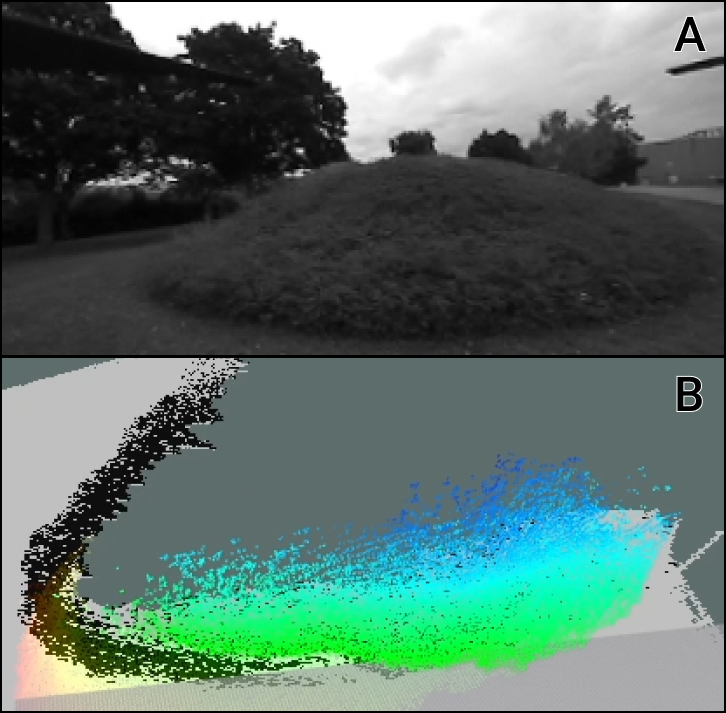
\includegraphics[width=0.5\linewidth]{img/MisalignedOdom}
	\caption{Resulting point cloud of unleveled camera with invalid odometry start data.\newline A: real life footage of the obstacle, B: tilted scan of the obstacle}
	\label{fig:custom_parts_misalignedOdom}
\end{figure}

\subsubsection{Design Process}

The solution to the aforementioned problems is a mount securing the ZED2i to the Matrice 100. Additionally to the specific characteristics, the mount has to fulfil, the ZED2i is the newest model with commercial products like mounts not being available. Therefore, to attain this custom mount design and manufacturing methods have to be used. 
The design portion is done with the help of CAD Software. CAD stands for Computer-Aided Design, meaning that rather complex designs can be realized in a short amount of time and less effort than doing it the traditional way. The software used in the autumn project is Fusion360, due to its option for a free license and previously acquired knowledge working with this software. 
The mount had to perfectly fit the camera to ensure the safety of the camera and drone. Therefore it is necessary to take measurements, which then are used to shape the design of the 3D model. In Fusion360 this can be best realized using parameterized design.

\begin{figure}[h]
	\centering
	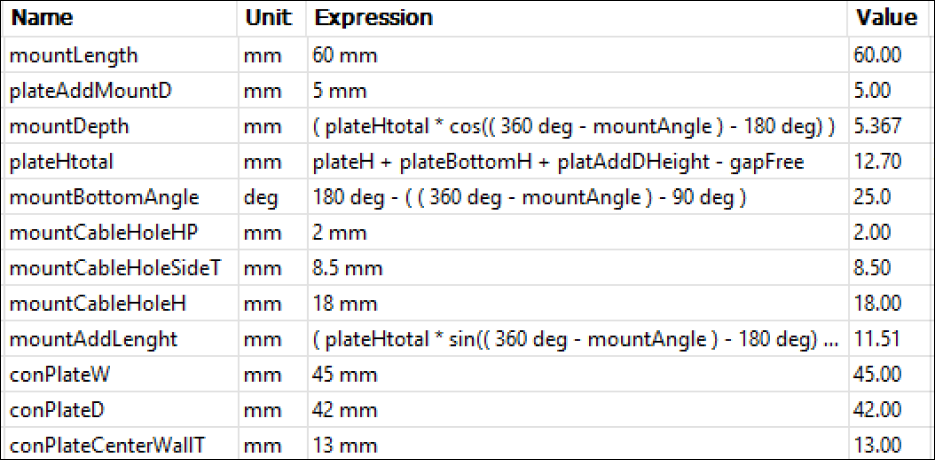
\includegraphics[width=0.7\linewidth]{img/Parameter}
	\caption{Excerpt of parameters used for the autumn camera mount design}
	\label{fig:custom_parts_parameter}
\end{figure}

Figure 11.3 depicts this concept of making the design dependent on parameters that can be easily adjusted. This allows for corrections to be made after the design process is finished. Without linking, sketches to parameters alterations would be time-consuming and would result in a model clouded with sketches overriding previous adjustments. Furthermore changes affecting complex areas in the part lead to artefacts, which when removed take more time than redesigning the part when applied to simple, one-component models, like the mount in autumn. An important property in the case of the autumn camera mount is the angle of the camera relative to the drone. This design principle makes it possible that changing the angle only means changing a number in a text field, which implies the change of several different dimensions of the part. 
Fusion 360 additionally comes with the capability of rendering the resulting model, in order to get a feel for how it would look in physical form.

\begin{figure}[h]
	\centering
	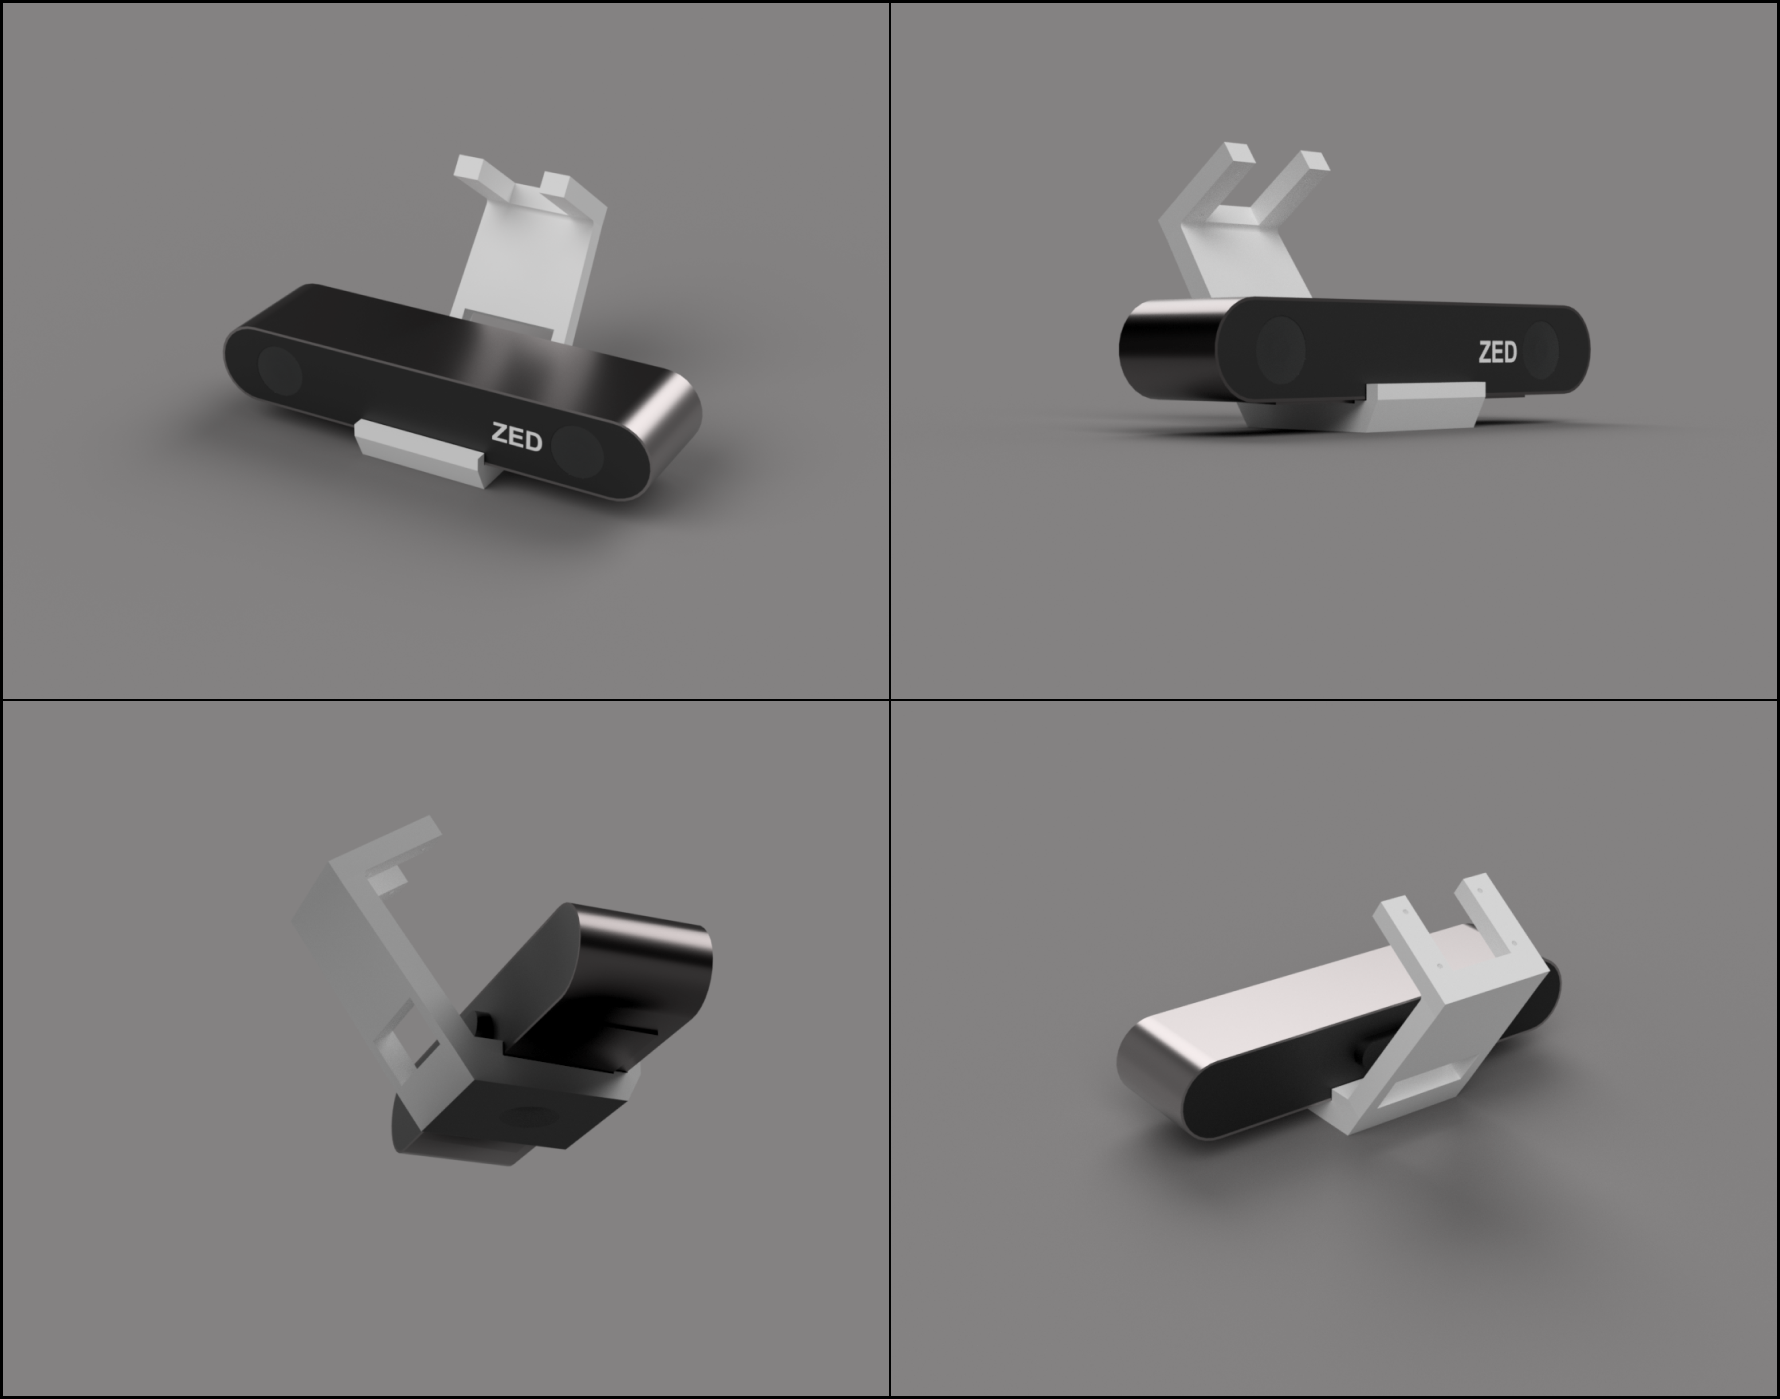
\includegraphics[width=0.6\linewidth]{img/MountRender}
	\caption{Render of the 3D-model for the camera mount attaching the ZED2i, also modeled and visible in the render, to the Matrice 100.}
	\label{fig:custom_parts_mountRender}
\end{figure}

\subsubsection{Manufacturing}

For the purpose of converting the 3D model to a physical object, the simplest and most time-efficient method is to utilize 3D printing. Nowadays 3D printing is a widespread technique to make ideas reality with little time and money. Therefore it is an optimal solution for the autumn project. 
When going from a 3D-modeled design to a 3D print a slicer is needed to convert the 3D object to code the printer understands. With most 3D printers printing in 2.5 dimensions, meaning that only the x and y-axis move freely while the z only adjusts its height once a layer is finished. This principle is reflected in the resulting file once a 3D model is sliced. The gcode consists of a header, defining settings for the print and a sequence of lines following it. A line of this gcode file would look like this: 
\[G1\ X120.95\ Y101.653\ E1.17355\]
The first part consists of the identifier $G$ and a number, marks which command should be executed. In the case of $G1$ it's "move in a straight line". Following the command, specifier are parameters, for this example the x and y end position is needed to draw a line. Additionally marked with the identifier $E$, is the flow rate defining how much filament is going to be extruded when moving to the given position.

The final step to attaining the physical form of a gcode file is printing it using a suitable 3D printer. Autumn uses a Creality Ender 5, because of its readability and print quality. Furthermore, the choice of the correct filament for a successful 3D print is needed. For a part, like a camera mount, which isn't under big stresses and no large forces are applied to it, filament-like acrylonitrile butadiene styrene, commonly known as ABS, isn't needed. Therefore the most widely used filament, polylactide is most fitted for this print.

\begin{figure}[h]
	\centering
	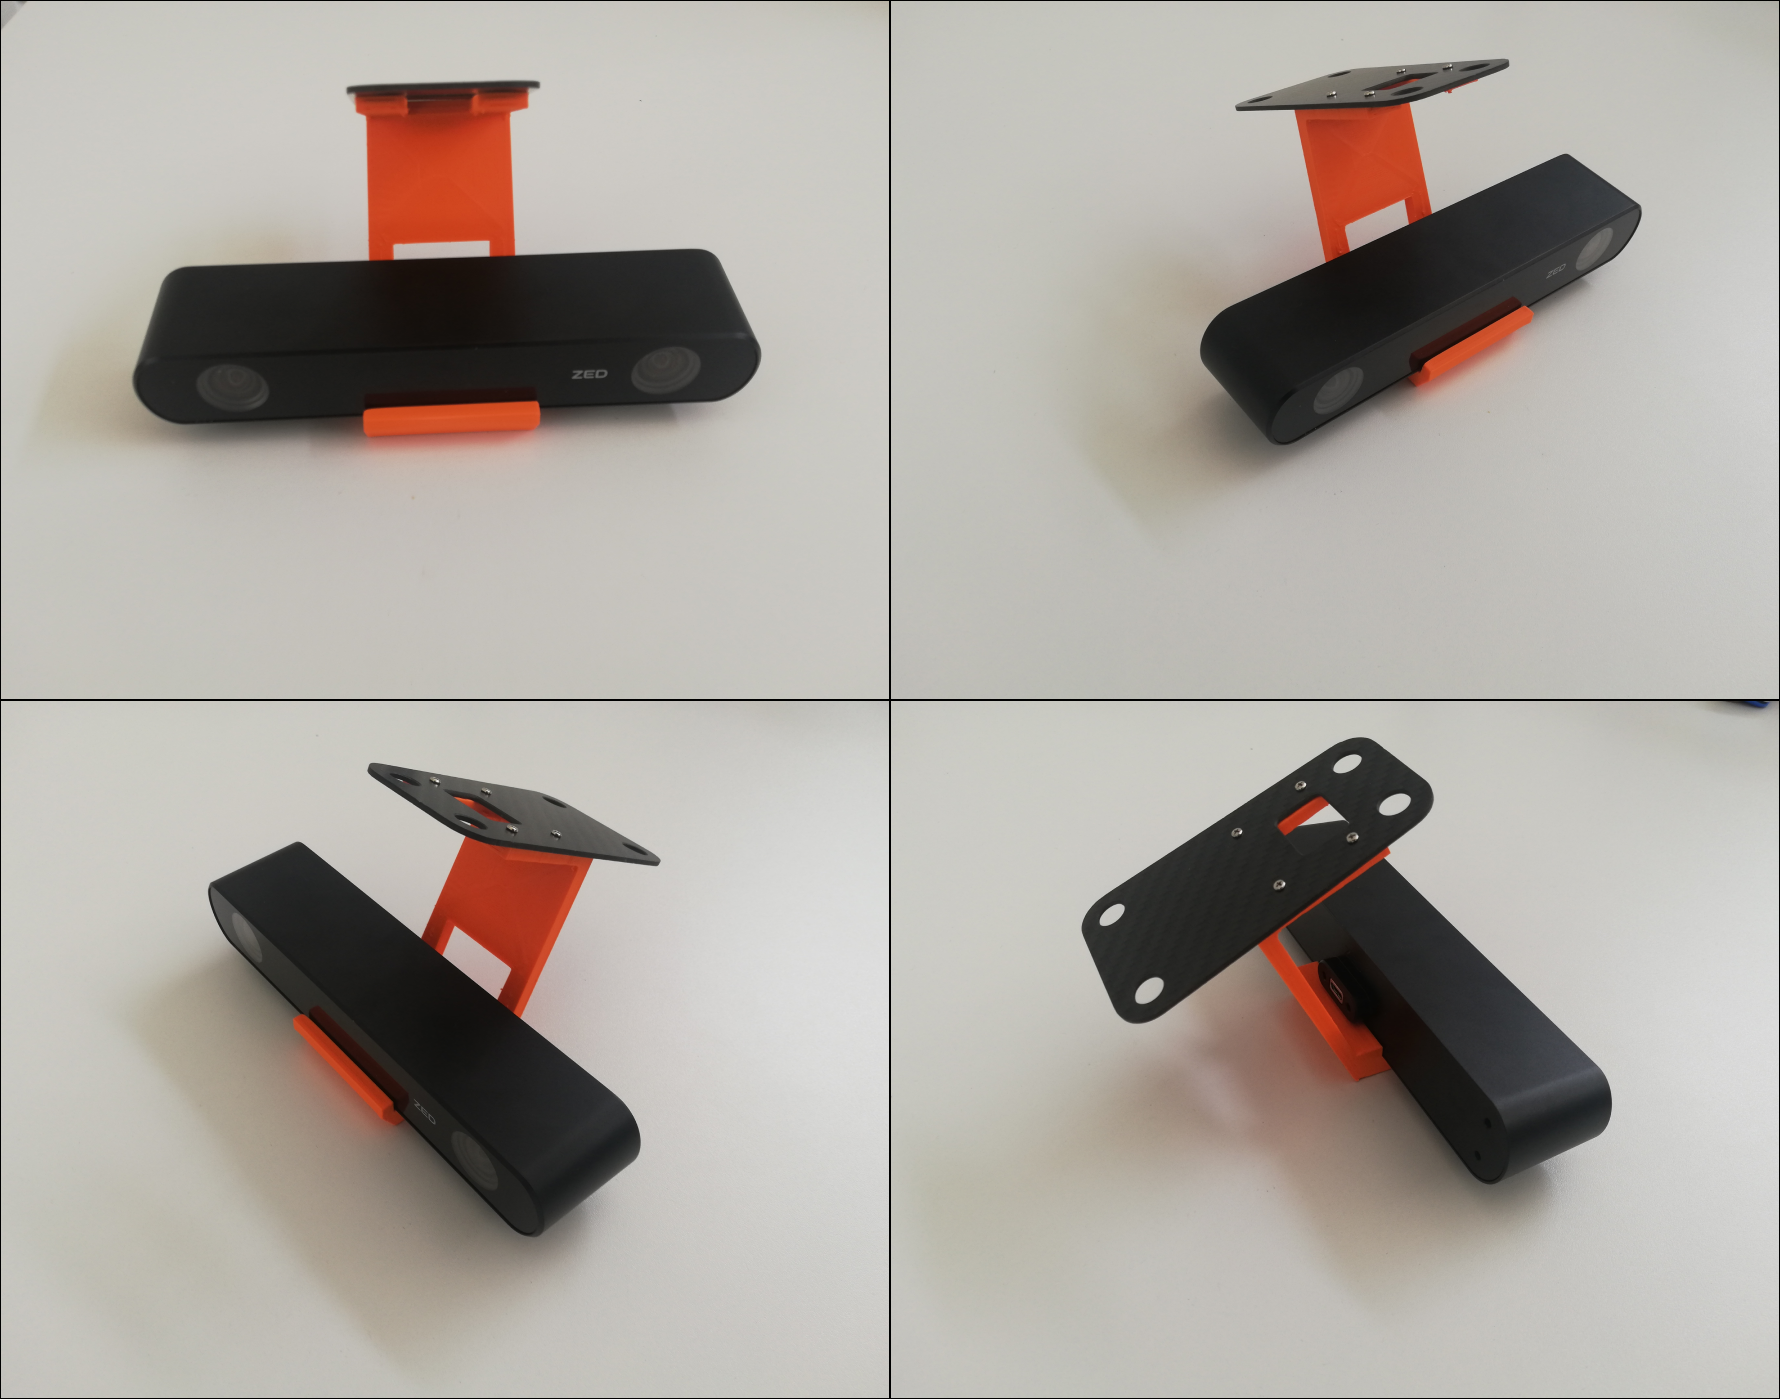
\includegraphics[width=0.6\linewidth]{img/MountPrint}
	\caption{3D-printed camera mount for the purpose of attaching the ZED2i to the Matrice 100. On top of the mount is the connection plate attaching on the drone.}
	\label{fig:custom_parts_mountPrint}
\end{figure}

\section{CAD Software}

This section is going to cover widespread CAD software solutions. Nowadays computer-aided design is an imperative principle, used in a variety of industries. CAD software improves the efficiency and quality of the design workflow. With free solutions being available, this industry standard has expanded to a clientele reaching from the leading companies to hobbyists creating innovation of the future in the comfort of their homes. Therefore when choosing an apt software, a multiplicity of properties have to be considered.

\subsection{SolidWorks}

SolidWorks being the industry-leading CAD solution, it is hard to overlook in a comparison. SolidWorks offers a fast array of functionality for not only CAD, additionally, but it also offers capabilities for computer-aided manufacturing. 
The target audience for SolidWorks is experts in the field of modelling and design. Hereby is not only the UI designed to cater more to a clientele that is firm in their understanding of the computer-aided design process, but also it offers more in-depth functionalities such as dynamic loading, linear and non-linear analysis and composite materials.\footcite{all3dpSolidWorksVsFusion2021}

\begin{figure}[h]
	\centering
	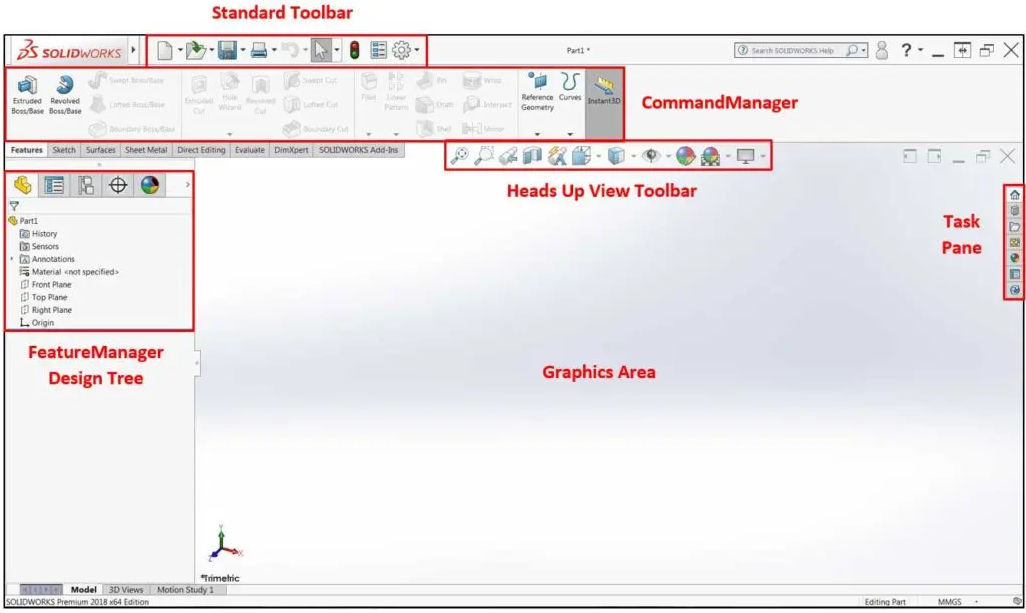
\includegraphics[width=0.6\linewidth]{img/SolidWorksUI}
	\caption{\citetitle{hawkridgesysUIBSolidWorks2019}}
	\label{fig:custom_parts_solidworks}
\end{figure}


\subsection{Fusion 360}

With Fusion 360 offering a non-commercial, free license option with limited functionality, it is widespread amongst the hobbyists and with its beginner-friendly UI design and possibility for an educational license with the majority of the functional scope of the professional license. Features included in the professional subscription that is excluded otherwise are mostly cloud processing options and load and stress simulations.

\begin{table}
	\centering
	\begin{tabular}{ |p{3cm}||p{6cm}|p{3cm}|  }
		\hline
		\multicolumn{3}{|c|}{Fusion 360 Licenses} \\
		\hline
		License & Features & Price\\
		\hline
		Fusion 360 for personal use& Standard design and 3D modeling tools& free\\
		\hline
		Fusion 360& Standard design and 3D modeling tools, plus a fully featured CAM, CAE, and PCB development platform& 495\$ p.a.\\
		\hline
	\end{tabular}
	\caption{An overview of Fusion 360 licenses with their respective capabilities and prices.\footcite{autodeskFusionPersonalNoDate}}
\end{table}

\subsection{Autumn choice}

When comparing the two CAD solutions, that are possibilities to be used in the autumn project, the most important characteristic is the user-friendliness in respect to the state of knowledge the user already has. Both SolidWorks and Fusion 360 offer more than enough functionality to fulfil the needs of autumn. When looking at the monetary dimension, where for the needed functionality Fusion has no competition with its free license for personal use. Furthermore is the Fusion 360 workflow tailored to the simple application, with a small number of components. SolidWorks follows an assembly based principle, in contrast, Fusion 360 is based on a multi-component architecture.\newline
In conclusion, due to the limited amount of functionality required from CAD software in the autumn project, Fusion 360 is being used.

\section{3D-Printing}

This section is going to focus on manufacturing methods available in the autumn project and compare them. Nowadays easy and fast prototyping is made possible with the use of 3D-printing technology. 3D-Printing has evolved over the years, away from a science fiction concept, to a widely used tool in part manufacturing, filling the gap left open by the geometrical limitations of conventional methods.\newline
Autumn having an area of competence, split between skills when working with soft- and hardware, it is important to have the means to manufacture custom parts, tailored to the needs of the project. With 3D-Printing being an affordable and accurate technology, in terms of translating virtual concepts to a physical object, it is an obvious choice to use for autumn.
When considering using 3D printing in any kind of project, it is important to think about which method is best fitted for the application.

\subsection{Fused Deposition Modeling}

FDM printing is the most commonly used and widespread method of 3D printing. The principle behind fused deposition modelling comprises using an extrusion device to eject a thermoplastic polymer. This polymer is heated to the point of its glass transition and consequentially extruded along a predefined path.

\subsubsection{Movement Variants}

The movement capabilities of 3D printers differ between two different approaches. Most desktop 3D printers are Cartesian-style 3D printers, which means it moves linearly in the x, y and z dimension.
Which parts of the printer move depend on the printer itself, commonly the print-bed moves in the y dimension, while the print-head covers x and the vertical z movement. In Contrast, the delta-printing method uses three vertical rods aligned in a triangle shape, to support the print-head and move it per individual movement of sledges, on the vertical rods, connected to the print-head.\footcite{all3dpFDM3DPrinting2020}\newline

\begin{figure}[h]
	\centering
	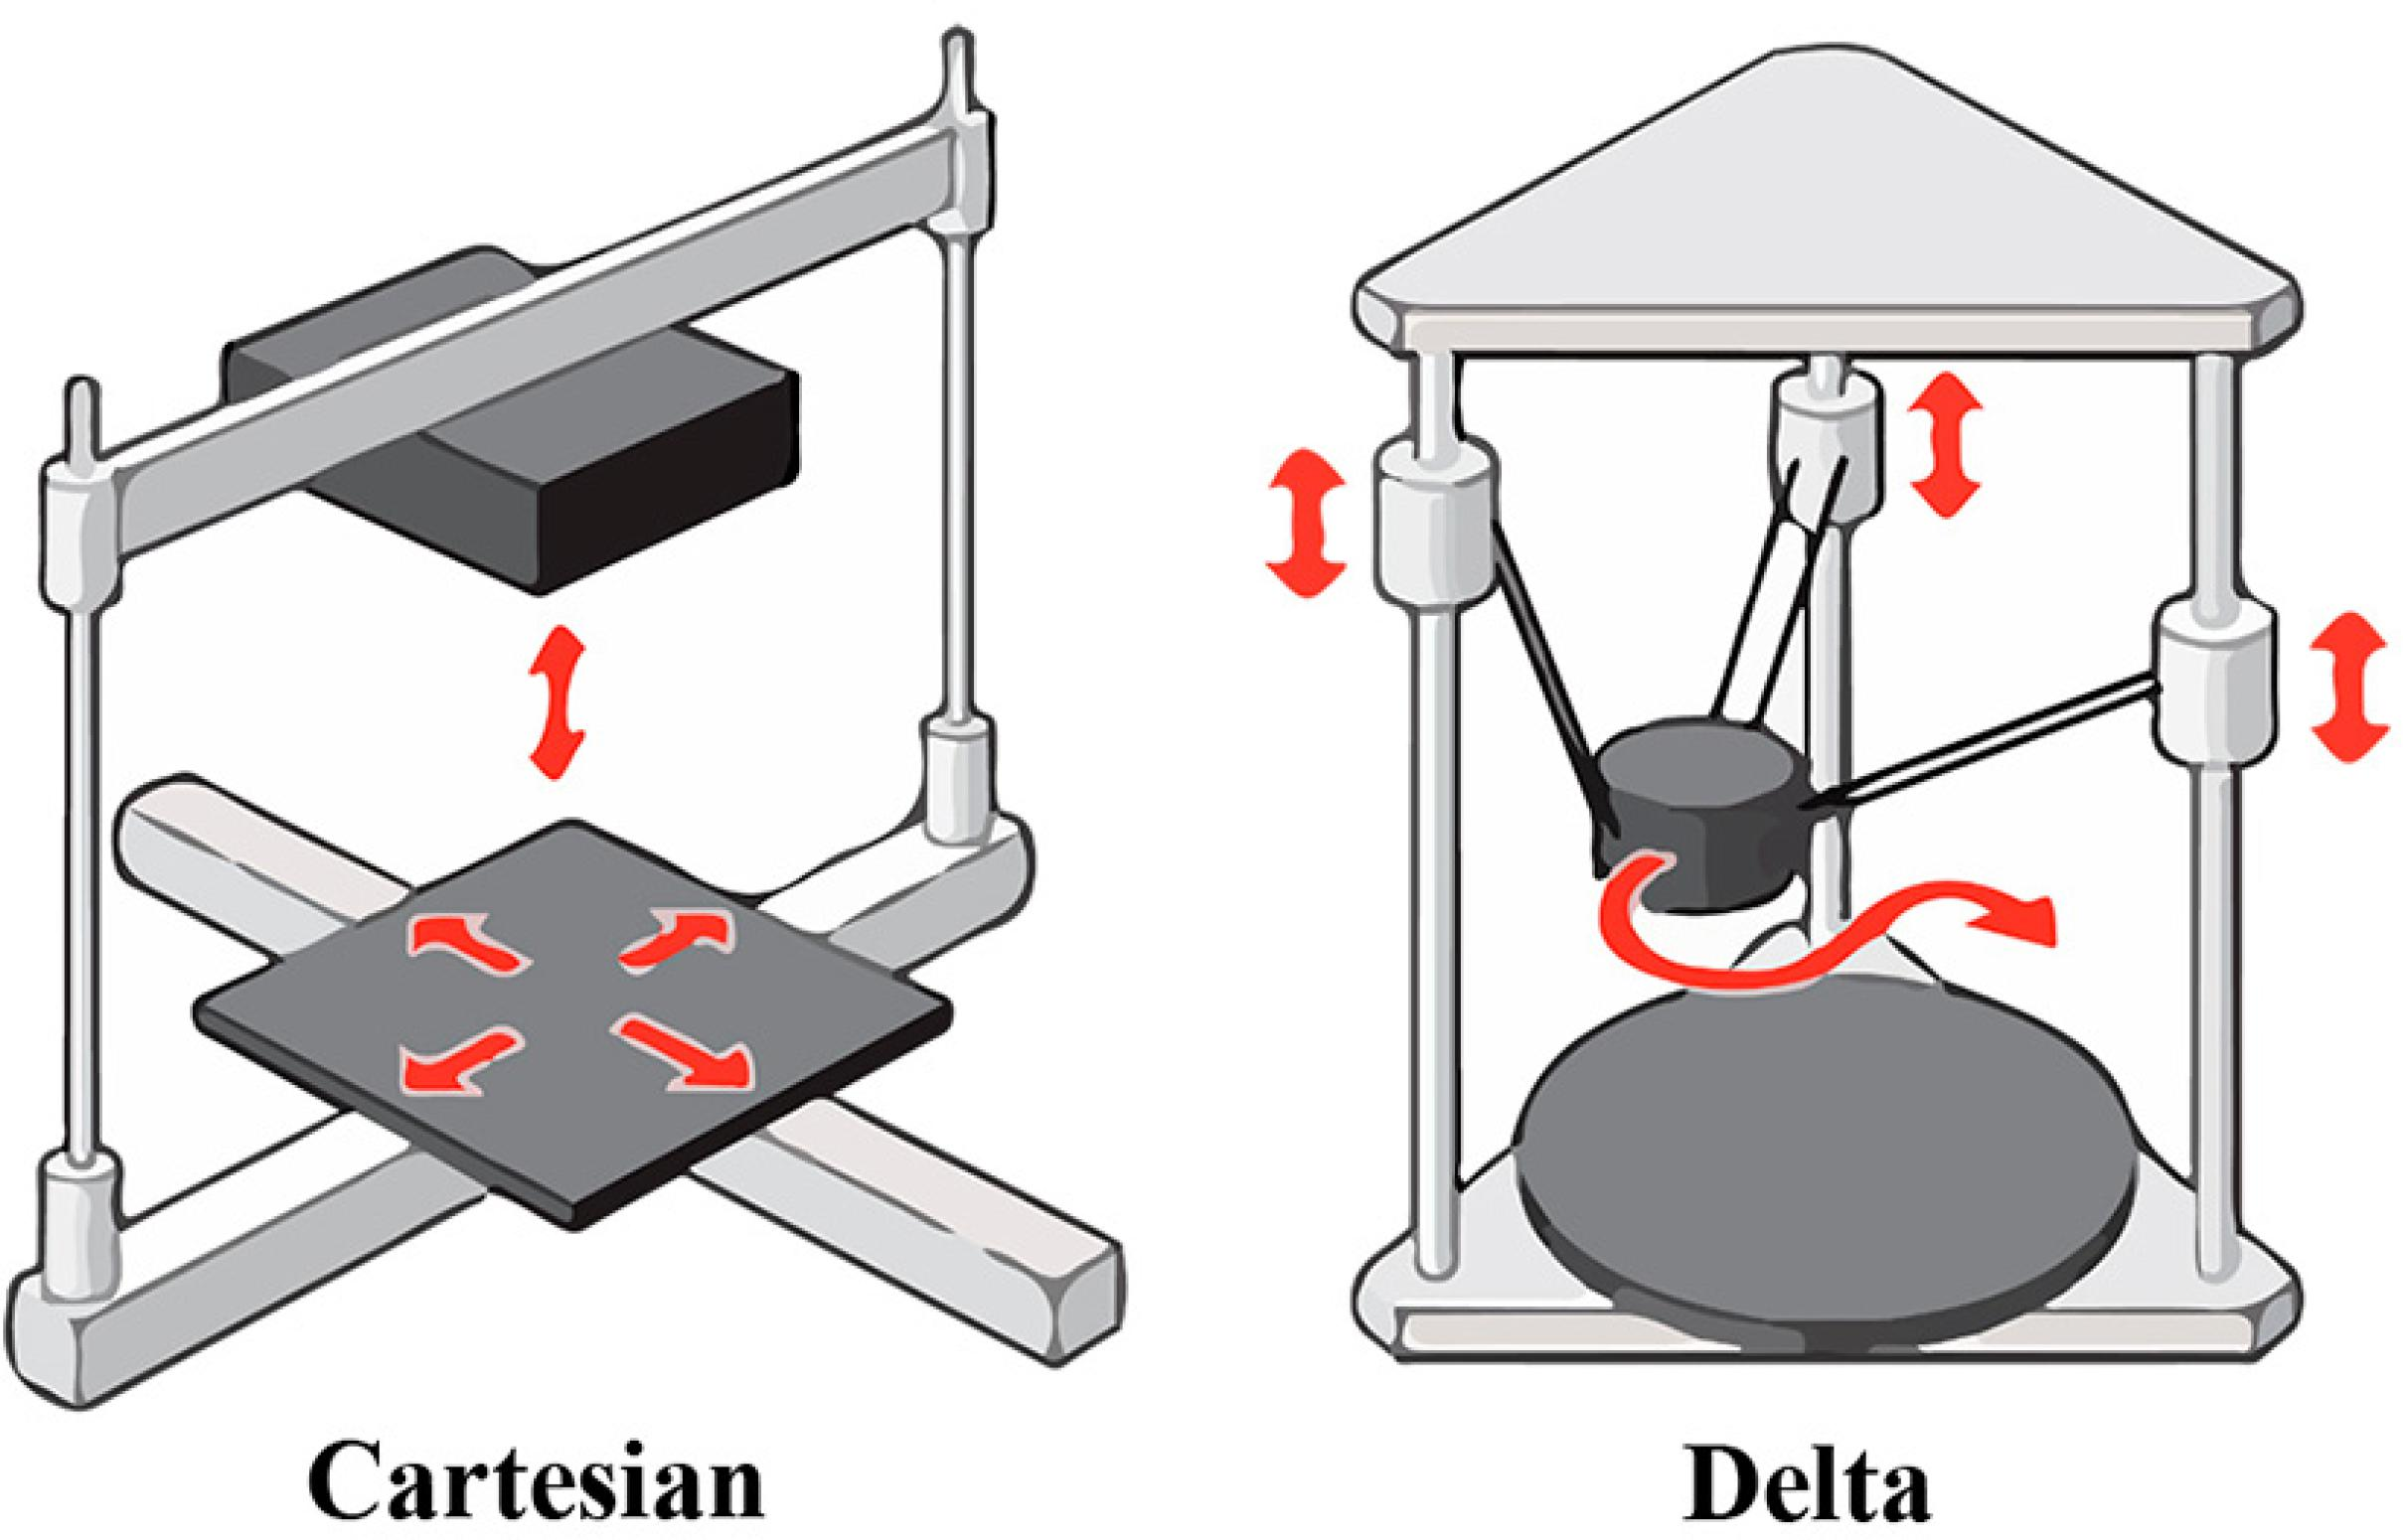
\includegraphics[width=0.6\linewidth]{img/cartesianDeltaPrinting}
	\caption{\citetitle{Schmitt2017}}
	\label{fig:custom_parts_printerMovement}
\end{figure}

Cartesian-style and Delta-style printers fundamentally contain the same parts. Both printer variants include a print-bed, print-head and stepper-motors, the difference is how they are arranged. Therefore the performance of these printing styles is similar and are more dependent on other factors than the movement system. The reason Cartesian-style printers are as popular as they are is due to the fact that the simpler Cartesian approach is user-friendlier and consumes less space, than its delta-style equivalent.\newline

\subsubsection{Main Parts}

In order to be able to distribute the filament according to the predefined path, calculated by the slicing software, components are needed, namely an extruder, hot-end, and nozzle. The extruder is used the feed the polymer to the print-head. The print-head itself consists of a hot-end and a nozzle, the hot-end is used to heat the thermoplastic polymer to the state of glass transition, after which it is forced through a nozzle and applied to either the print-bed directly or on top of another layer.\footcite{all3dpFDM3DPrinting2020}


\begin{figure}[h]
	\centering
	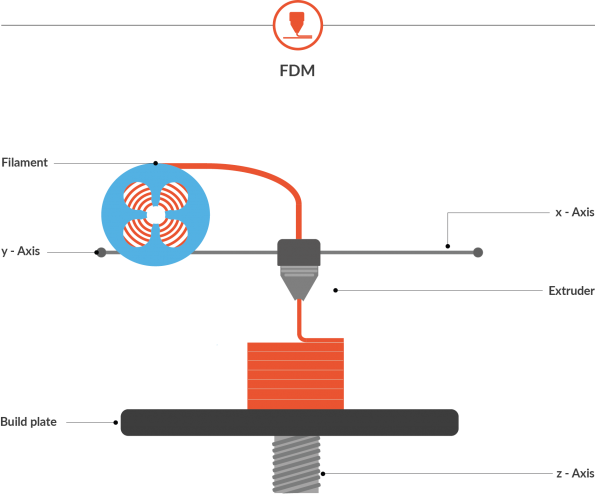
\includegraphics[width=0.5\linewidth]{img/FDM_Principle}
	\caption{\citetitle{druckwegeFusedDepositionModelling}}
	\label{fig:custom_parts_fdm_parts}
\end{figure}

\subsubsection{Filament}

The aspect of the filament used for a print heavily influences the success and usability of a part. The most common filaments include PLA, ABS and Nylon. PLA is the easiest to work with, it is the most frequently used, when needing a more robust material than PLA a suitable polymer would be ABS. Cases, where Nylon is used, are when highly flexible parts are desired.\footcite{hubsIntroToFDM3DPrintingNoDate}


\subsection{Stereolithography}

SLA is known for its accuracy and detail in conjunction with 3D printing. SLA-printers use a photosensitive resin in combination with a laser to construct a part. This allows printers using this method to keep mechanical components to a minimum. In contrast to FDM printing, SLA uses thermoset polymers, which leads to parts being irreversible once printed. FDM printed parts will melt, when exposed to heat, SLA printed parts don't turn back to liquid, instead they start to burn.\footcite{hubsSLA3DPrintingNoDate}

\subsubsection{Printing process}

At the start of every print, depending on the printer design, the build-plate is positioned, so that one layer height of resin is present between the build-plate and laser. Thereafter the beam from the UV laser is redirected to cure a layer according to the information given by the slicer. In order to add the third dimension, the build plate moves a distance of one layer height every time a layer is finished. This process is repeated until the final layer.\newline
After the part is finished, it is in a still not fully cured state. To fully cure a part further exposure to UV light is needed, this step is happening in a so-called curing station. \footcite{hubsSLA3DPrintingNoDate} 

\subsubsection{Design Variants}

SLA printers are divided into two different designs. For desktop use printers are built with a bottom-up architecture, which means the build-plate is attached to a so-called elevator. Therefore the light source is placed below the vat containing the resin. This design allows for affordable prices, by sacrificing build volume.\newline
In industrial applications, top-down designs are used. By placing the build plate into the vat, it enables larger build volumes.\footcite{hubsSLA3DPrintingNoDate}

\subsection{Autumn choice}

In Autumn parts are designed to be practical, which entails a simple geometry. Therefore in terms of accuracy, it wouldn't be advantageous to use an SLA printing method. Furthermore, in regard to structural integrity, both parts printed with FDM and SLA printers are sufficient for the stresses parts are exposed to in the Autumn use case. With Autumn being focused on fast prototyping and fast iteration, SLA with its extensive curing process would be unfit with no benefits gained from using a Stereolithography style printer. 

